\section{Protect yourself}

\begin{center}
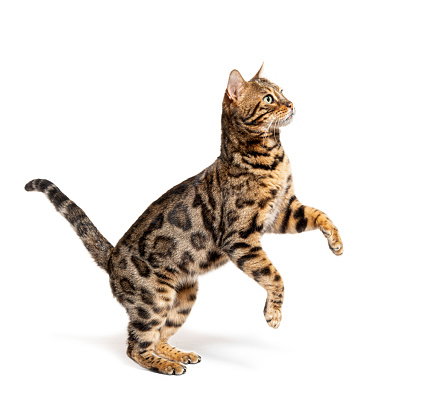
\includegraphics[width=6cm]{images/15_protect.jpg}
\end{center}

\begin{textit}
Should we protect ourselves? And from what?

My cat sits on the windowsill. It's about two meters to the top book shelf that he wants to jump on. He takes aim.

He evaluates.

He checks out different points of view.

He wriggles on his spot.

Then he vigorously jumps... and lands.

Elegantly.
\end{textit}

A participant explains to me that she cannot come to the practice evenings because there are always these "intense energies and she needs to protect herself from them".

I don't say anything.

It is not the right moment to reasonably ask whether some "other" energies are really "out there", or if it might be a product of our own perception of the mind. If I assume that there are monsters underneath my bed, I will also find them there.

I myself don't believe that I have to protect myself, at least not beyond a reasonable amount, which prevents me from being hit by the very first truck on the street. Of course I too am afraid sometimes. I too have read the news, have my childhood traumas, went through quite a few unfortunate experiences and huge disappointments and know roughly what can happen in life.

But to protect myself by not exposing myself to life and its challenges, surprises and contradictions would mean that, in fact,  I cut myself off from my own (!) life. And that would be even worse than what possibly could happen.

Yes, to encounter people can be exhausting. And it is true that executing tasks can lead to frustration. We can also agree that saying yes or no to the other person can lead to rejection. No matter what I do, I expose myself to the danger that something can go wrong. Of course we want to safeguard ourselves from that, to protect ourselves! We can achieve that by retreating into a safe cave, or \ldots

\ldots or we can protect ourselves by encountering those scary experiences with open eyes and open arms, embracing them.

Should we evaluate the situation? Of course!

Should we strive for the best solution? For sure!

Should we think thoroughly, to give myself advice? Hell yes!

But then jump vigorously!

Like the cat.

Because the fear of life and the need to protect myself from all those scary things can only be discarded by having trust in life and myself. And that is only achievable by doing precisely those things I feel a bit scared of.
